\chapter{制冷}
\section{引言}
制冷对超导非常重要。对制冷的依赖性是超导广泛应用(如电力应用)的主要因素。然而,我们不以因为其重要性而过分强调它的作用。
单从制冷角度看,显然将超导磁体运行于最高的许可温度下是更高效的。但是,如果超导磁体是某系统的一部分,就必须评估运行温度对整个系统的影响。
“超导磁体的最佳运行温度”这个问题就成了现实且极端重要的设计/运行问题,对高温超导磁体尤其如此。比如,对运行于77K的超导磁体,如果产生
相同的磁场,无疑需要比运行于20K更多的超导体;制冷上的节省可能并不能补偿超导体费用的增加。

另一个不可忽略的是每一个超导系统的绝热要求:最好的绝热是真空。温度低于20K(氢的冰点)时,热学“有效”的真空在低温容器内是相对容易实现的。
已抽真空的低温容器表面逸出的氢气是容器内最主要的传热介质。于是,整个高温超导磁体系统若运行于20K之下(而不是之上)可能经济性更好。
如果我们选择一个更高的运行温度——比如很多人希望的~70K——系统中可能不再需要真空绝热,这时“干扰”又少了一点。

本部分,将简要讨论以下超导磁体的制冷设计、运行问题:1)两种超导体的冷却方式,“干式”和“湿式”;2)冷源、热源和制冷测量;
3)湿式磁体的制冷剂;4)可能对干式磁体有用的固体制冷剂。上述论题的更多细节将在“专题”部分有更深入的涉及和研究。

\section{“湿式”磁体和“干式”磁体}
在1990s前,所有的超导磁体都是“湿式”的,即靠液氦冷却。1990s早期开的,随着高温超导的发现以及制冷机技术的进步,由制冷机冷却的干式(无制冷剂)
LTS和HTS磁体都得以发展。一方面,干式低温系统在运行、维护上更轻便;另一方面,干式低温系统更易实现“少干扰”。这使得干式磁体在多数应用中是更优的
选项——如果磁体自身在正常运行条件下完全无耗散(如交流损耗)的话。

\subsection*{超导磁体的冷却方式}
如表4.1可见,超导磁体可以使用五种冷却方式(四种湿式和一种湿式)的任一种。尽管本节使用的“制冷??”、“绝热”、“准稳定性”等术语
在第六章会有更详细的讨论,但为了读者的可理解性,此处给出这些术语的简要定性解释。
\begin{description}
  \item[浸泡冷却cryostable?] 1980s以前建造的磁体基本都是浸泡式冷却的。这些磁体的一个关键制冷特征是为了便于制冷剂渗入的绕组的“通孔”设计。
  通孔让绕组的几乎所有部分都暴露于制冷工质。此时,下文定性讨论的对流传热是重要的。第六章会给出一些数据。
  \item[浸泡冷却绝热] 为了实现高性能,浸泡冷却的“绝热”磁体在1980s早期开始发展。此处,绕组是实心的,完全没有制冷剂的浸入。
  这样,绕组中的总体电流密度显著高于浸泡制冷??。绕组仅在其外表面被冷却。
  \item[迫冷cryostable] 为了保持制冷剂为单相(一般对浸泡式制冷磁体并不容易),以及为了加强绕组导体本身的强度,在1970s早期发展了所谓的“cable-in-conduit,CIC,特别是大型磁体”。此处,冷却和绕组高度耦合。重要的传热数据是哪些强迫对流参数。典型的传热数据在第六章给出。
  \item[迫冷准稳定性] 为了保持绕组鲁棒性,绕组上没有通孔。为实现比浸泡冷却绝热磁体更好的稳定性,制冷剂被强迫进入绕组。不是经由导体,而是
  仅在导体的临近边缘。和绝热绕组一样,导体是传导冷却的。
  \item[制冷机冷却] 磁体和制冷机相连;绕组内的冷却主要通过传导。如第六章将会更详细讨论的,LTS磁体运行于准稳定态,而HTS磁体运行于稳定态。
  “制冷循环器(cryocirculator)”对作为干式磁体冷源的制冷机是非常需要的,特别是对LTS磁体。
\end{description}
%%%表4.1
\begin{table}[htbp]\small
  \centering
  \caption{湿式和干式超导磁体的冷却方式} \label{coolingmethod}
\begin{tabular}{|c|c|c|}
  \hline
  % after \\: \hline or \cline{col1-col2} \cline{col3-col4} ...
\textbf{冷却方式}&\textbf{冷却-导体耦合性}&\textbf{传热方式} \\ \hline \hline
浸泡冷却,cryostable & 好;全部导体& 对流\\ \hline
浸泡冷却,绝热 & 基本不存在 &(磁体绕组表面的)传导 \\ \hline
迫冷,cryostable &好;全部导体&对流\\ \hline
迫冷,准稳定 &临近表面处,间接&传导\\ \hline\hline
制冷机,准稳定&间接 &传导 \\ \hline
\end{tabular}
\end{table}

\section{制冷问题:冷却、热、测量}
三个基本制冷问题是与超导磁体技术相关的:1)冷源;2)热源;3)测量。这些问题将在本部分简要讨论。专题部分以及后续章节将对某些特定问题
做更详细的讨论。
\subsection{冷源}
如表4.1总结的,超导磁体靠制冷工质或制冷机冷却并维持在其运行温度。下面将简明的讨论制冷剂。制冷机仅给出基本的热力学关系和性能数据。
\subsection{热源}
一般的,在超导磁体的低温容器内的冷环境中,主要有五个热源:1)低温容器壁间的辐射;2)低温容器壁间“真空”空间的热对流;3)磁体支撑和
低温容器结构单元的热传导;4)电流引线的传导和焦耳热耗散;5)磁体内的耗散。专题部分将会涉及到辐射、对流和电流引线。磁体的耗散将在第七章讨论。
\subsection{测量}
超导磁体运行中,通常测量的低温参数包括:1)温度;2)压力(低温容器真空度、工质压力);3)工质流速(迫冷湿式磁体);4)蒸发率(湿式磁体的电流引线)。本书中,专题部分仅涉及温度的测量简要讨论。

\section{液体工质:湿式磁体}
1990s前,仅液氦适用于磁体运行。某些液氦低温容器使用液氮来隔断热量。由于磁体要从室温冷却到4.2K,液氮也用于预冷液氦冷却磁体,以减少液氦的消耗。

大气压下饱和(沸腾)温度低于100K的6种工质是:氧(90.18K)、氩(87.28K)、氮(77.36K)、氖(27.09K)、氢(20.39K)、氦(4.22K)。
对于湿式高温超导磁体和设备,工质的备选顺序为氮、氖、氢。对于湿式低温超导或低温/高温混合磁体,如高场NMR磁体,仍然主要使用氦。五种
液体的沸腾热传递参数在表4.2列出。作为对比,还列出了水的参数。

%%表4.2
\begin{table}[htbp]\small
  \centering
  \caption{沸腾传热参数} \label{boilingpara}
\begin{tabular}{|c||c|c|c|c|c|}
  \hline
  % after \\: \hline or \cline{col1-col2} \cline{col3-col4} ...
\textbf{液体}&$T_a[K]$&$h_l[J/cm^3]$&$q_{pk}[W/cm^2]$&$\Delta T_{pk}[K]$&$q_{fm}[W/cm^2]$ \\ \hline \hline
氦&4.22&2.6&$\sim 1$&$\sim 1$&$\sim 0.3$\\ \hline
氢&20.39&31.3&$\sim 10$&$\sim 5$&$\sim 0.5$ \\ \hline
氖&27.09&104&$\sim 15$&$\sim 10$&$\sim 1$\\ \hline
氮&77.36&161&$\sim 25$&$\sim 15$&$\sim 2$\\ \hline
水&373.15&2255&$\sim 100$&$\sim 30$&$\sim 10$ \\ \hline
\end{tabular}
\end{table}

\subsection*{沸腾传热参数}
在湿式超导磁体中,特别是浸泡冷却cryostable磁体,冷却依靠核态沸腾传热。由于核态沸腾传热中,冷却是靠液体蒸发实现的,故液体的体积蒸发热$h_l$
是一个关键参数。这也意味着沸腾热流密度和温度的关系图像(两坐标轴均为对数坐标,如图\ref{boilingflux})对大多数液体都是看上去类似的。这里的x轴温度是浸入
液体的物体的避免温度和液体饱和温度之差,即$\Delta T=T-T_s$。图中的其他参数为:$q_{pk}$,最大核态沸腾热流密度;$\Delta T_{pk}$,是$q_{pk}$出现时的$\Delta T$;$q_{fm}$,最小膜态沸腾热流密度。

从表\ref{boilingpara}中我们可以得到,唯一适合LTS磁体的制冷剂液氦,蒸发时吸收的能量密度最小,是效果最差的。尽管HTS磁体最好是干式运行,但如果它湿式运行,
氢、氖、氮能够覆盖大多数HTS磁体的温度范围。燃料电池在电动汽车领域应用中发展出的一个重要成果就是液氢技术,包括安全性方面的技术。这可能会为
液氢冷却HTS磁体提供与有益促进。

%%%图4.1
\begin{figure}
  \centering
 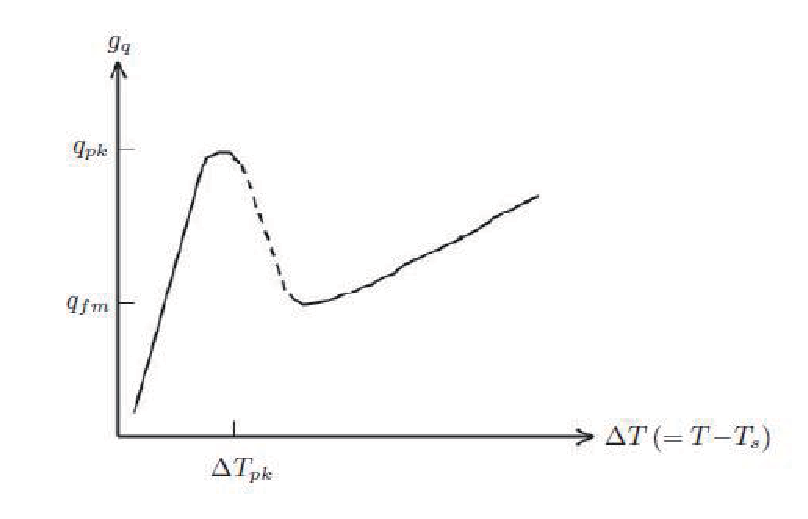
\includegraphics[scale=0.8]{chpt4/figs/fig4.1.eps}
  \caption{典型流体的沸腾热流密度 vs. 温度}\label{boilingflux}
\end{figure}

\section{固体工质:干式磁体}
正如前文所讲,干式低温磁体,特别是运行电流小于1kA的,很可能会逐渐替代湿式小电流LTS磁体。如果当前的高温超导体(BSCCO、YBCO和$MgB_2$)中
的一种、两种甚至三种发展为完全的“磁体级导体”,那在不久的将来,干式HTS磁体不仅会取代干式LTS磁体,还将找到仅适用于HTS磁体的其他应用。
\subsection{湿LTS磁体 vs. 干HTS磁体——热容}
湿式LTS磁体经常被忽略的一个优势是其巨大的热容,这是由作为湿式LTS磁体的一部分的大量液氦提供的。液氦的焓密度在4.2K时“高”达$2.6 J/cm^3$——
此处所谓高,是和铜相比的。铜在4.2-4.5K的焓密度仅为$\sim 0.0003J/cm^3$——是铜的1000倍。于是,在大多数情况下,液氦将牢牢将磁体的温度“铆”住。

干式磁体同样需要提供一个大的热容以便“铆”住温度。固态制冷剂是这种功能的很好选项。图\ref{fig:heatcap}给出了多种固体制冷剂(固氖、固氮、固氩)以及
部分金属(铅、银、铜)的热容和温度的关系。铅在低温设备中常用为热容增强部件;铜是LTS中广为使用的基底金属;银是BSCCO的基底金属。
%%%图4.2
\begin{figure}
  \centering
 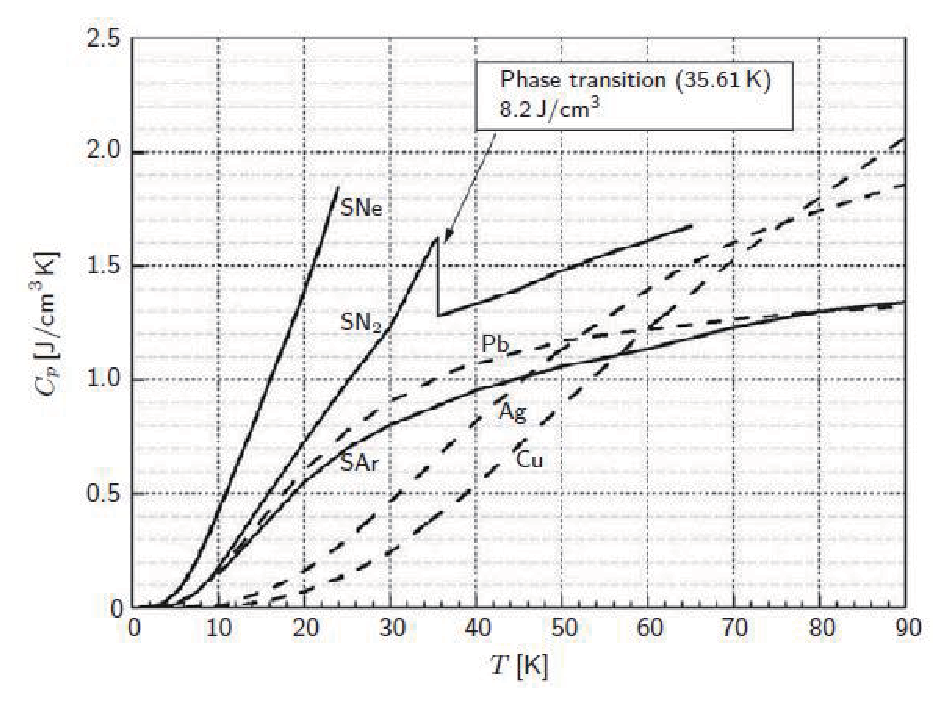
\includegraphics[scale=0.7]{chpt4/figs/fig4.2.eps}
  \caption{几种物质的热容$C_p$ vs. 温度T特性}\label{fig:heatcap}
\end{figure}

\subsection{固体工质——氖、氮、氩}
下面将简要讨论三种可能用于干式HTS磁体的固体工质:氖、氮、氩。附录中给出了他们的一些热力学性质。

尽管是高热容使得固体工质成为优秀的浸渍材料。此外,还有两个其他的性质让固体工质在一些应用中优于环氧:1)热导率;2)机械强度。在10-15K温度区间,
在HTS绕组上的温度均匀性上,固氮比环氧的效果更好。同时,固氮也使得绕组比环氧浸渍更具鲁棒性。

\begin{description}
  \item[固氮,$SN_2$] 因为它能在高达64.2K仍保持固态且不贵、重量很轻(铅的密度的1/10)、具有电绝缘性,固氮是运行于64K温度下温区的干式HTS磁体的
  有效热容增强剂。例如,BSCCO和YBCO磁体在20-60K温区肯定能运行;$MgB_2$磁体则是在10-15K甚至20-30K。从图4.2中看出,固氮在35.61K存在一个
  固-固态的相变,额外吸收能量$8.2J/cm^3$。由于在转变点古今的热容是约$1.5J/cm^3 K$,额外的$8.2J/cm^3$能量吸收等价于5K多的温升。对于运行于
  这个温区的HTS磁体,这是一个极佳的“温度池”。
  \item[固氖] 图4.2中的热容数据表明,固氖体积费用比固氮贵200倍,它将是4-10K温区的最佳热容增强剂。不过,10K左右时,固氮对于大多数情况就足够用了。
  尽管也有其他物质,比如$Er_3 Ni$,在4-24K温区能提供更好的热容增强效果。但是对磁体,固氖可能更合适。除了价格之外的最大缺点(相比于固氮),是
  固氖相对低的熔点,仅24.6K。这限制了固氖系统运行的温区。
  \item[固氩] 作为大气中含量最高的惰性气体,氩在价格上比氖至少便宜 一个数量级,不过比氮还是贵不少。固氩仅适用于运行于64.2K(固氮熔点)
  -83.8K(固氩熔点)温区的干式磁体。
\end{description}

\section{专题}
\subsection{问题4.1:Carnot制冷机}
因为超导电性发生在很低温度,所以需要制冷机来实现并维持低温环境。
使用图4.3所示的Carnot制冷机,我们来研究用于制冷的最高效率的热力学过程。
Carnot制冷机由两个可逆绝热过程和两个可逆等温过程组成,工质流体在两个热源之间运行,
从而最高效率的做功。尽管Carnot效率实际中是不能实现的,但它给出了可能的上限。

a) 在$T$ vs. $S$图上画出Carnot循环。使用图4.3中标出的记号。$T_{op}$:冷源温度,一般等于磁体运行温度;
$S_{cl}$:离开冷源的工质的熵;$T_{wm}$:高温热源的温度;$S_{wm}$:进入高温热源的工质的熵。冷源和热源的温度$T_{op}$和$T_{wm}$都是常数。

b)证明,对于理想Carnot制冷机,为了从热源$T_{op}$中提取热量$Q$并将其释放到$T_{wm}$中,需要的输入功$W_{ca}$为:
\begin{equation}% 4.1
W_{ca}=Q(\frac{T_{wm}}{T_{op}}-1)
\end{equation}

c)证明,高温热源为$T_{wm}=300\ \mathrm{K}$的Carnot制冷机,在$T_{op}=4.2\ \mathrm{K}$时,$W_{ca}/Q\simeq 70$;
在$T_{op}=77\ \mathrm{K}$时,$W_{ca}/Q\simeq 3$。
\begin{figure}[htbp]
	\centering
	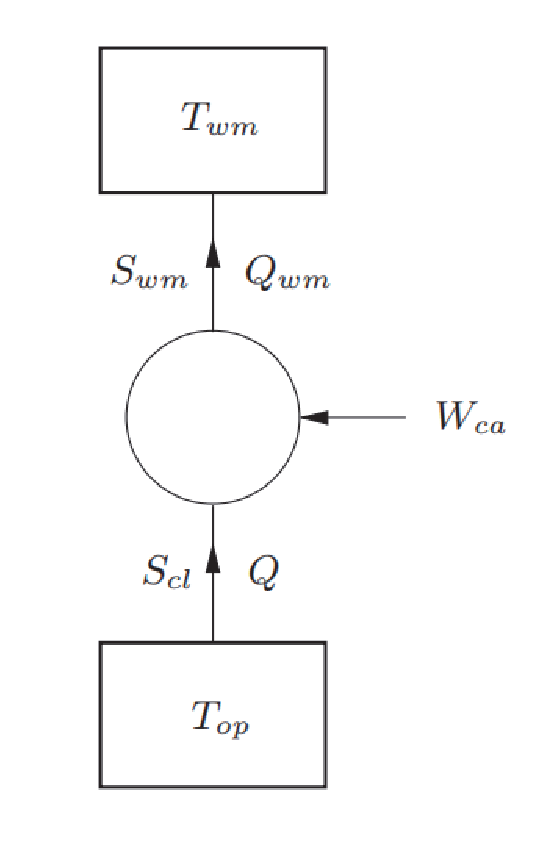
\includegraphics[scale=0.5]{chpt4/figs/fig4.3.eps}
	\caption{工作于两个热源之间的Carnot制冷机。}
\end{figure}

\subsubsection{问题4.1之解}
a) Carnot制冷机工作于两个热源之间,从低温热源$T_{op}$中提取热量$Q$,然后向高温热源$T_{wm}$释放热量$Q_{wm}$。
如图4.3所示,制冷机的运行需要功$W_{ca}$。

Carnot制冷循环由工质的四个可逆过程组成,如图4.4的$T$ vs. $S$图所示:
\begin{itemize}
	\item 工质的等熵压缩,开始于状态1($S_{wm},T_{op}$);
	\item 等温压缩,开始于状态2($S_{wm},T_{wm}$);
	\item 等熵膨胀,开始于状态3($S_{cl},T_{wm}$);
	\item 等温膨胀,开始于状态4($S_{cl},T_{op}$),结束于状态1。
\end{itemize}

b)热力学第一定律:
\begin{equation*}% S1.1
Q_{wm}=Q+W_{ca}=0 \tag{S1.1}
\end{equation*}

式中,$W_{ca}$是制冷机的输入功,等于$T$ vs. $S$图上的闭合面积(当图4.3中的$W_{ca}; Q; Q_{wm}$方向相反时,
Carnot循环代表理想做功机,$T$ vs. $S$图上的闭合面积表示输出功)。
因为每个过程都是可逆的,有$Q=T_{op}(S_{wm}-S_{cl})$和$Q_{wm}=T_{wm}(S_{wm}-S_{cl})$。有:
\begin{align*}% S1.2a
S_{wm}-S_{cl}&=\frac{Q}{T_{op}}\tag{S1.2a}\\
S_{wm}-S_{cl}&=\frac{Q_{wm}}{T_{wm}}\tag{S1.2b}
\end{align*}

令上面两个式子相等,有:
\begin{equation}% S1.3
\frac{Q}{T_{op}}=\frac{Q_{wm}}{T_{wm}} \tag{S1.3}
\end{equation}

联立S1.1和S1.3,有:
\begin{equation*}% S1.4
\frac{Q}{T_{op}}=\frac{Q+W_{ca}}{T_{wm}} \tag{S1.4}
\end{equation*}

解出S1.4中的$W_{ca}$,得到:
\begin{equation*}% 4.1
W_{ca}=Q(\frac{T_{wm}}{T_{op}}-1) \tag{4.1}
\end{equation*}

\begin{figure}[htbp]
	\centering
	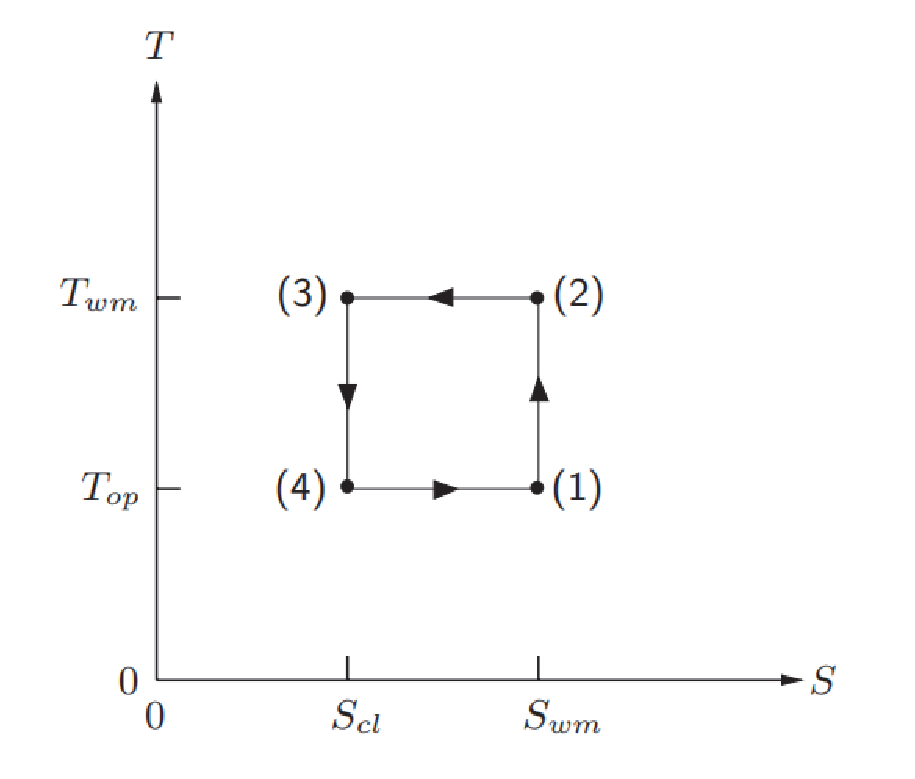
\includegraphics[scale=0.4]{chpt4/figs/fig4.4.eps}
	\caption{Carnot制冷机的$T$ vs. $S$图。}
\end{figure}

c)\textbf{$4.2–300\ \mathrm{K}$温区}:在$T_{op} = 4.2\ \mathrm{K}, T_{wm} = 300\ \mathrm{K}$
时,从方程4.1可得$W_{ca}/Q\simeq 70$;也就是说,4.2 K的1 W制冷量,需要制冷机70 W的输入功。
实际制冷机中,性能比定义为$W_{ca}/Q$($W_{cp}$是压缩功)随着$Q$增大而提高。
小单元($Q=1\ \mathrm{W}$)大概$\sim 10,000$,大单元($Q\sim 100\ \mathrm{kW}$)在$\sim 300$。

\textbf{$7.7–300\ \mathrm{K}$温区}:将$T_{op} = 77\ \mathrm{K}, T_{wm} = 300\ \mathrm{K}$
代入方程4.1,可得$W_{ca}/Q\simeq 3$;实际制冷机性能比在$\sim 50$(小单元,$1\ \mathrm{W}$)到$\sim 10$(大单元,$\sim 100\ \mathrm{kW}$)之间。

\subsection{讨论4.1:制冷机性能}
这里,我们简要从两个不同的角度看一下制冷机的性能:
1) 单一额定功率下的制冷机在不同运行温度下($Q/T_{op}$);
2) 组合额定功率下和运行温度,但运行在不同温度下。

\textbf{A. 特定温度下的特定制冷功率}

图4.5给出的是特定制冷功率$Q$($\mathrm{W}$)下的$W_{cp}/Q$vs. $T_{op}$关系曲线[4.19]。
图中的$\otimes$符号表示Carnot循环。
\begin{figure}[htbp]
	\centering
	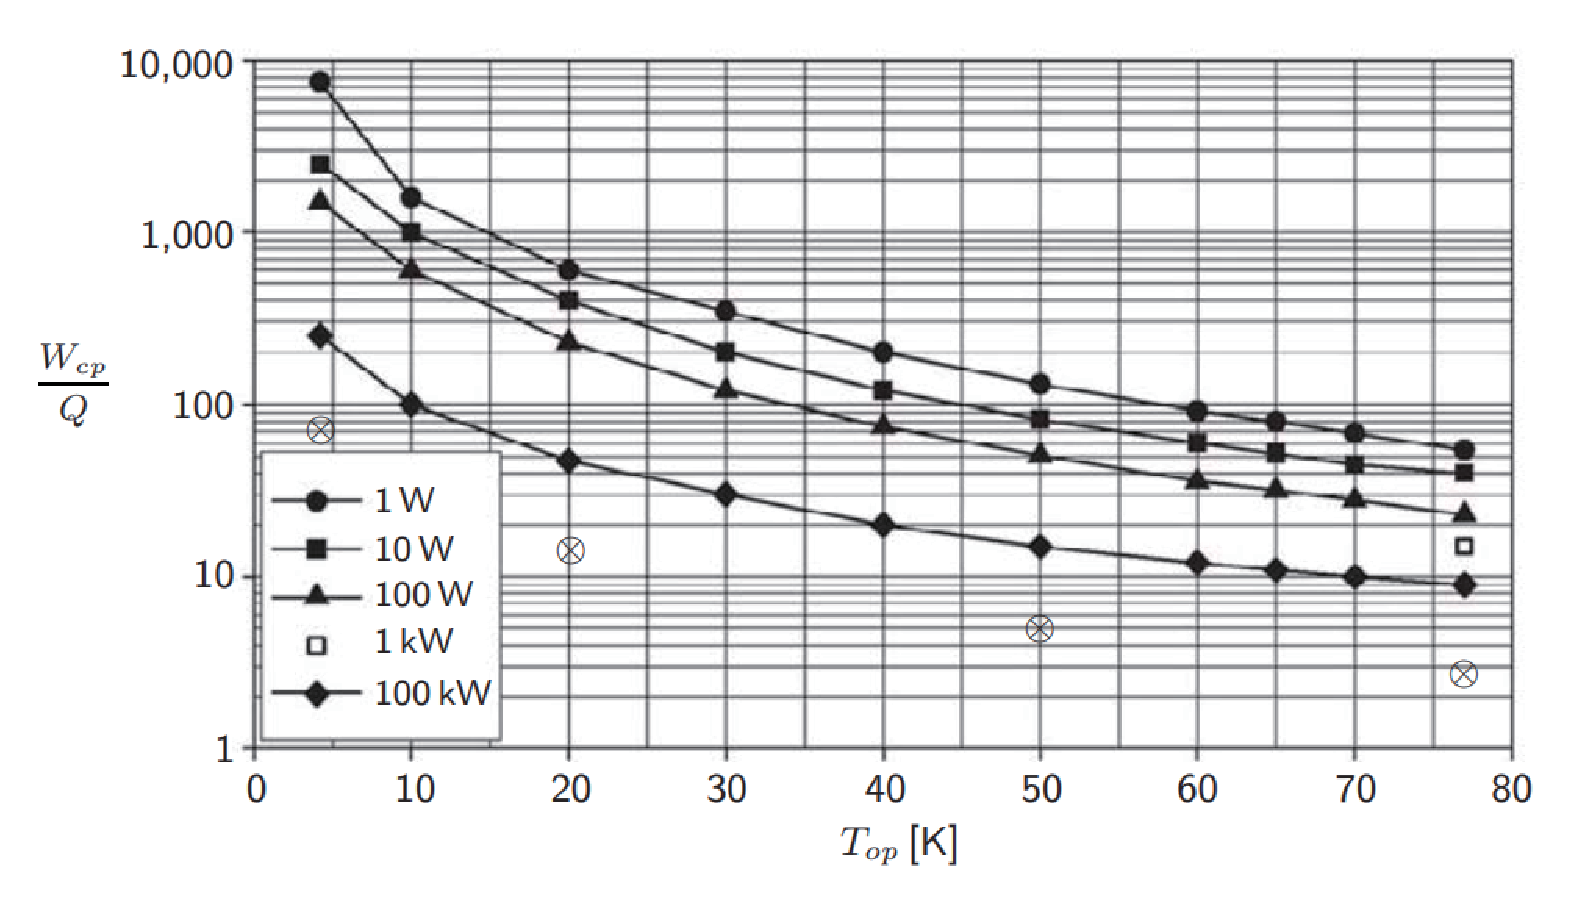
\includegraphics[scale=0.4]{chpt4/figs/fig4.5.eps}
	\caption{特定制冷功率$Q$($\mathrm{W}$)下的$W_{cp}/Q$vs. $T_{op}$关系曲线。$\otimes$符号表示选定温度下的Carnot循环,计算时取$T_{wm}=300\ \mathrm{K}$。}
\end{figure}

这样,对一个设计运行温度$T_{op}=4.2\ \mathrm{K}$的1 W制冷机(实心圈)的$W_{cp}/Q$是7500;
对运行温度$T_{op}=20\ \mathrm{K}$的1 W制冷机,$W_{cp}/Q$是600。
下面将论及,在特定温度4.2 K和20 K下优化的制冷机在不同温度区间$T_{op}$下的$W_{cp}/Q$是不同的。

\textbf{B.在非设计温度下的运行}

\begin{figure}[htbp]
	\centering
	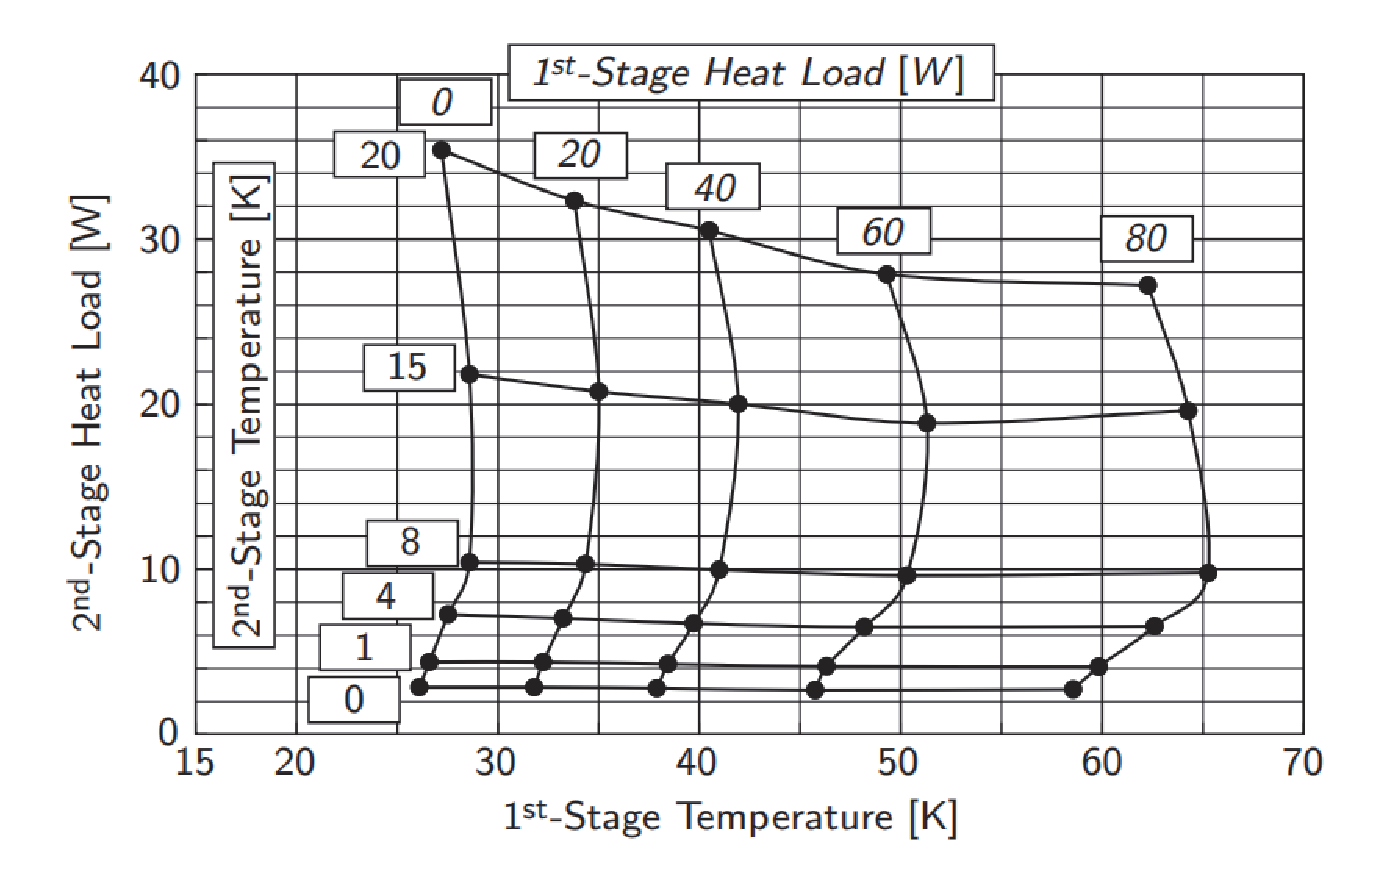
\includegraphics[scale=0.5]{chpt4/figs/fig4.6.eps}
	\caption{二级制冷机的性能数据。}
\end{figure}

图4.6给出了一台二级制冷机(住友重工Model RDK-408D2)的性能(一、二级制冷功率)数据,
性能是作为第一级和第二级运行温度的函数给出的。
它的标称最低二级运行温度是4.2 K,此时的制冷功率$Q=1\ \mathrm{W}$需要压缩功率$W_{cp}=7.5\ \mathrm{kW}$,
也即$W_{cp}/Q = 7500$。数据给出了制冷机在同样的压缩功率下的二级功率/温度比:从3 K时的0W,即$W_{cp}/Q = \infty$,到
20 K时的15 W,即$W_{cp}/Q = 500$。 (图4.5表明,一个15 W/20 K单元在20 K优化后的$W_{cp}/Q$大约是350。)
那些在给定二级温度为大约20 K时近乎水平的二级制冷线表明,在一级温度处于$\sim 25-\sim 60\ \mathrm{K}$区间时二级制冷功率几乎与之无关。

因为制冷机的压缩功率7.5 kW与一二级负荷无关,为了维持二级温度在一个理想水平,
总的热负荷,至少是二级的热负荷,必须匹配其制冷功率。
这样,如果二级运行温度希望是20 K——一级运行条件为 40 W/42 K——如果二级的实际热负荷是5 W,
那必须给二级提供额外的10 W的热负荷。因为如图4.6所示,二级在20 K提供15 W的制冷功率。
这个额外的10 W热负荷一般由附属于二级冷头的加热器产生,这会导致系统效率的降低。


\subsection{讨论4.2:湿磁体的冷却模式}
因为从体积上讲,LH2不仅在价格上比LN2至少贵一个数量级,而且其汽化潜热也仅是LN2的$\sim 1/60$。
LHe冷却的磁体通常经过两个步骤冷却:1)用LN2将磁体冷到77 K;2)从低温容器中吹除LN2,然后立即使用LHe继续冷却磁体。
对一个大型磁体 (>1吨),步骤2中的LN2将被减压至0.14 atm以改变其温度,此时的磁体会达到64 K。

\textbf{“理想”模式}

理想冷却模式下,磁体在一系列无限小的与冷氦气的理想能量交换中冷却。在第$n^{th}$步中,$T_n$的磁体被冷却至$T_n-\Delta T$,
$\Delta M_{he}$的液氦汽化,被加热到$T_n$。氦气在温度$T_n$和室温之间的可用焓并未用于冷却磁体。
如果$M_{he}$是将一个重为$M_{mg}$的磁体从$T_i$冷却至4.2 K所需的液氦质量,那么有:
\begin{equation}% 4.2
\frac{M_{he}}{M_{mg}}=\int_{4.2K}^{T_i}\frac{c_{cu}(T)dT}{h_{he}(T)-h_{he}(4.2K,liq.)}
\end{equation}

式中,$c_{cu}(T)$是铜的比热(表示绕组中的所有材料),$h_{he}(T)$是氦的比焓。

这个冷却模式实际不可能实现,但通过向磁体下面的低温容器空间非常缓慢的引入液氦的方法可以逼近理想模式。
不过,冷却速率不能任意的慢,因为那会耗费太长的时间,消耗大量的液氦去抵消低温容器的热泄露。

\textbf{“浸泡”模式}

冷却的一个极端模式是浸泡初始温度为$T_i$的整个磁体到温度为液氦沸腾温度4.2 K的容器中。在浸泡模式下,
从$T_i$冷却磁体至4.2 K,有$[M_{he}/M_{mg}]_{dk}$:
\begin{equation}% 4.3
\left[\frac{M_{be}}{M_{mg}}\right]_{dk}=\frac{[h_{cu}(T_i)-h_{cu}(4.2K)]}{h_L}
\end{equation}

式中,$h_L[\mathrm{kJ/kg}]$是LHe在4.2 K的汽化比热。$h_{cu}(T_i)$和$h_{cu}(4.2\ \mathrm{K})$分别是铜
在两个温度下的比焓。

\textbf{辅以LNe或LN2的冷却}

对于运行温度$T_{op}\ge 10\ \mathrm{K}$的制冷机冷却的HTS磁体,有时候要求以比单独用制冷机更快的速度将磁体从室温冷却到
$T_{op}$。我们用两步来满足这个需求:1) 如果$T_{op}<27\ \mathrm{K}$,使用液氖(LNe)达到27 K;如果$27\ \mathrm{K}<T_{op}<77\ \mathrm{K}$,就用液氮;2)用制冷机冷却到$T_{op}$。
上述两种制冷模式下需要的LNe或LN2量,可以由方程4.2或者4.3来计算,只是代入Ne或N2的焓值即可。

表4.3给出了液体制冷工质(LHe, LNe, LN2)在“理想”模式和“浸泡”模式下将1000 kg铜块从$T_i$冷却至4.2 K(LH2)、27 K(LNe)、77 K(LN2)分别所需的体积(以“升”计)。同时还给出了铜的比焓$h_{p_{cu}}$数据。
从表4.3,我们可以清晰的看到,对一个LH2冷却的磁体,采用LN2预冷极大的节省了LH2。
很明显,几种制冷工质的体积汽化潜热的巨大差异——LHe的2.6[$\mathrm{J/cm^3}$],LNe的104[$\mathrm{J/cm^3}$],LN2的161[$\mathrm{J/cm^3}$]——决定了所需的体积量。

\colorbox{red}{表4.3}



\subsection{讨论4.3:“制冷机冷却”HTS磁体}
本节我们研究一个干式HTS磁体,它由制冷机将其从初始温度$T_i$经过一个总的冷却时间$\tau_{cu}$冷却至运行温度$T_{op}$。
这个制冷机的二级冷却功率$Q_r(T)$与其温度$T$的关系见图4.7。
我们看到,这台制冷剂的制冷功率额定值是10 W@10 K(它的一级用来冷却磁体周围的辐射屏)。

为了简化讨论,我们考虑一个仅由磁体和制冷机组成的绝热控制体,系统冷却期间无额外热输入。
同时,我们假定磁体由铜块$M_{cu}$代表。
铜的热容$C_{cu}[\mathrm{kJ/m^3}]$图见附录III,该图基于铜密度为常数,即$\rho_{cu}=8960\ \mathrm{kg/m^3}$。
进一步我们假定冷却速率足够缓慢,在整个冷却期间,铜(磁体)的温度$T_{cu}$在整个绕组总是均匀的,并且总是等于制冷机的温度$T$,即$T_{cu}=T$。

在这个包含制冷机和质量为$M_{cu}$的铜(磁体)的控制体上应用热力学第一定律,并注意到$T_{cu}=T$,有:
\begin{equation}% 4.4
-Q_r(T)=\left(\frac{M_{cu}}{\varrho_{cu}}\right)C_{cu}(T)\frac{dT}{dt}
\end{equation}

方程4.4中$Q_r(T)$的符号表示制冷机提供的是制冷:磁体(铜块)正在冷却,即$dT/dt<0$。

\begin{figure}[htbp]
	\centering
	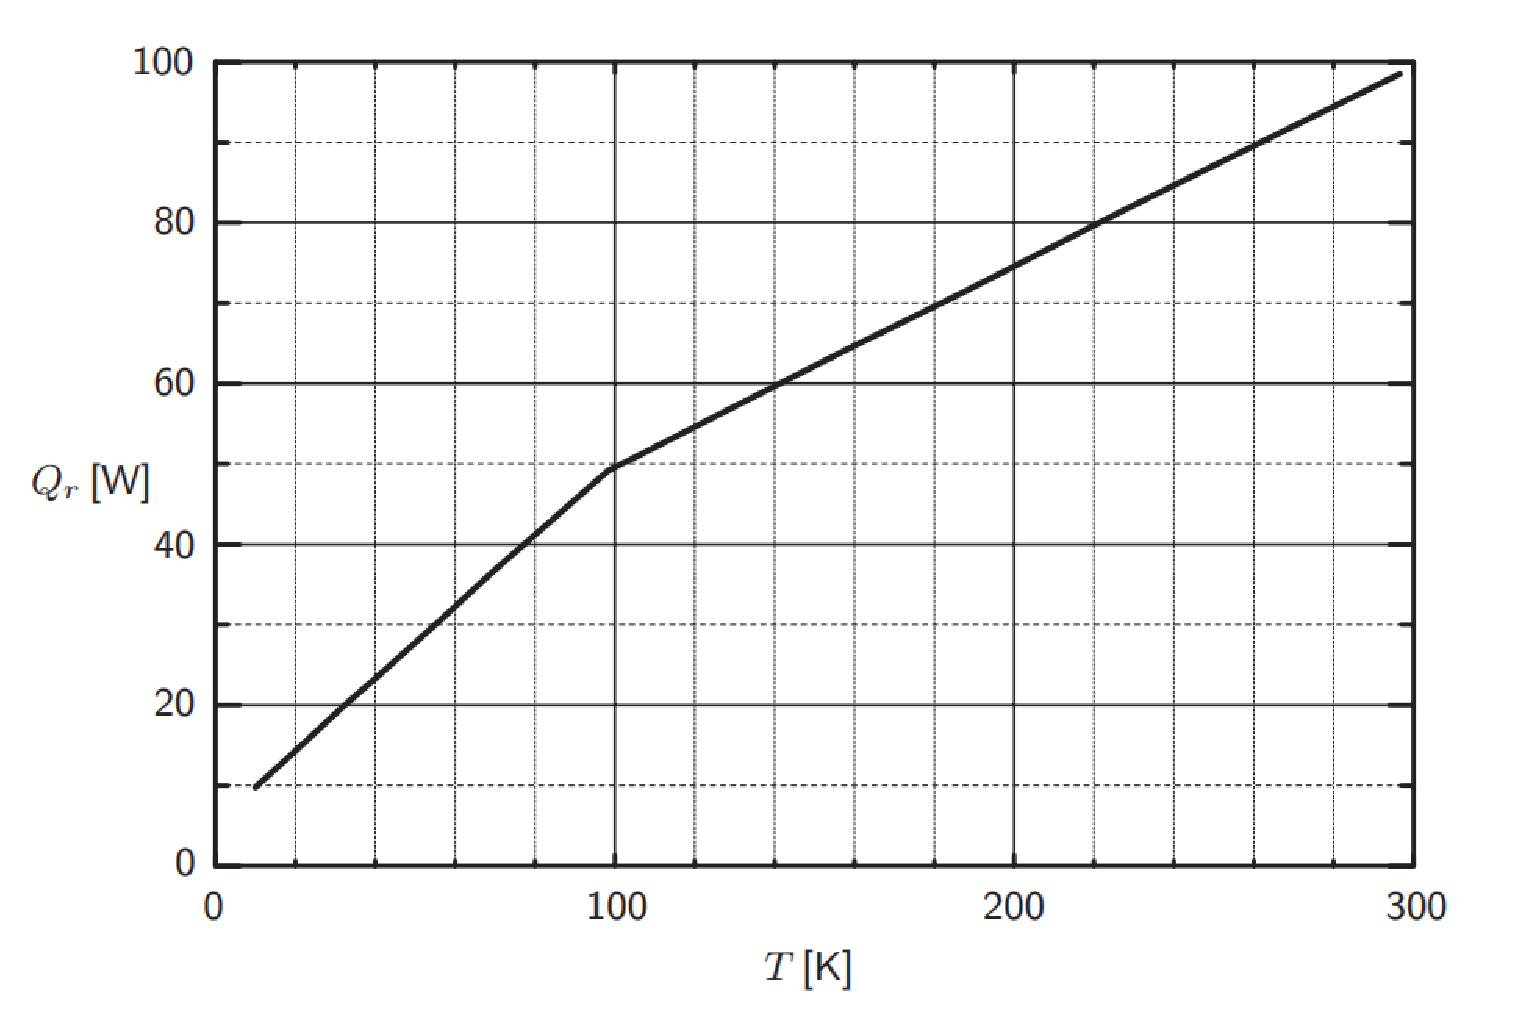
\includegraphics[scale=0.5]{chpt4/figs/fig4.7.eps}
	\caption{磁体制冷机的$Q_r(T)$曲线。}
\end{figure}
	
\colorbox{red}{表4.4}

表4.4列出了$Q_r(T)$,$C_{cu}(T)$和$\kappa(T)\equiv C_{cu}(T)/Q_{r}(T)$在给定温度下的值。
我们可以通过积分方程4.4,在特定的$T_i,T_{op},Q_r(T),M_{cu}$组合下解出$\tau_{cu}$:	
\begin{subequations}% 4.5
\begin{align}
\tau_{cn}&=\frac{M_{cu}}{\varrho_{cu}}\int_{T_{op}}^{T_i}\frac{C_{cu}(T)}{Q_r(T)}dT=\frac{M_{cu}}{\varrho_{cu}}\int_{T_{op}}^{T_i}\kappa(T)dT\\
M_{cu}&=\frac{\varrho_{cu}\tau_{cn}}{\int_{T_{op}}^{T_i}\kappa(T)dT}
\end{align}
\end{subequations}

在一些应用中,$\tau_{cu}$是主要的设计要求。可以看出,方程4.5b限制了在$\tau_{cu}$内可以冷却下来的铜的质量$\~{M}_{cu}$(这里代表磁体质量)。
对于给定的$T_i$和$T_o$组合,$\~{M}_{cu}$正比于$\tau_{cu}$。
表4.5给出了以图4.7中给出的$Q_r(T)$为基准的$T_i$,$T_o$和$\tau_{cu}$组合下的$\~{M}_{cu}$。
这样,如果磁体经4个小时从300 K冷却至30 K,受限的冷却质量是11.6 kg。

表4.5给出的结果清晰的指出了对于给定的$\tau_{cu}$,如果我们首先将磁体冷却至77 K,将可以极大的增加$\~{M}_{cu}$。
表4.3可以用于估计实现这个过程的所需LN2量。

\colorbox{red}{表4.5}


\subsection{讨论4.4:超流}
图4.8是常规氦($He^4$)的相图,其中给出了两种流体形式He I和He II[4.20]。
因为He II有独特的超高热导($k$)和超低黏性($\nu$)的独特性质,它被称为超流氦。
我们从相图中可以看出,沸点为4.22 K的常规氦 (He I)通过简单的加压即可变为He II。
当达到饱和压力5 kPa (37.8 torr)后,液体在2.18 K称为超流。
2.18 K被称为$\lambda$点,记为$T_\lambda$。
根据二流体模型,超流的比分在$T_\lambda$时为零,而随温度降低单调增加。
通过对比He II和常见物质的物性,我们可以看到超流氦的热导和黏性的独特性(表4.6)。

\textbf{传输性质}

因为超流氦的超高热导率,它常被用作超导磁体的制冷工质,通常运行于$\sim 1.8\ \mathrm{K}(<T_\lambda)$。
(尽管我们这里使用热导率的经典定义,即热导$\propto$温差。
在He II中,温差越小,等效热导率越大。等效热导率同样依赖于热通量。)
He II的搞热导率不允许液体中存在足以引起汽化的温度梯度。
这样,不像运行于4.2 K的He I冷却的磁体绕组,1.8 K的He II冷却的“无气泡”绕组不需要通道。
不过,这并不意味着He II可以在窄通道内无限制的传输热流。
类比于超导体中的临界电流,He II有一个临界热流密度。

\begin{figure}[htbp]
	\centering
	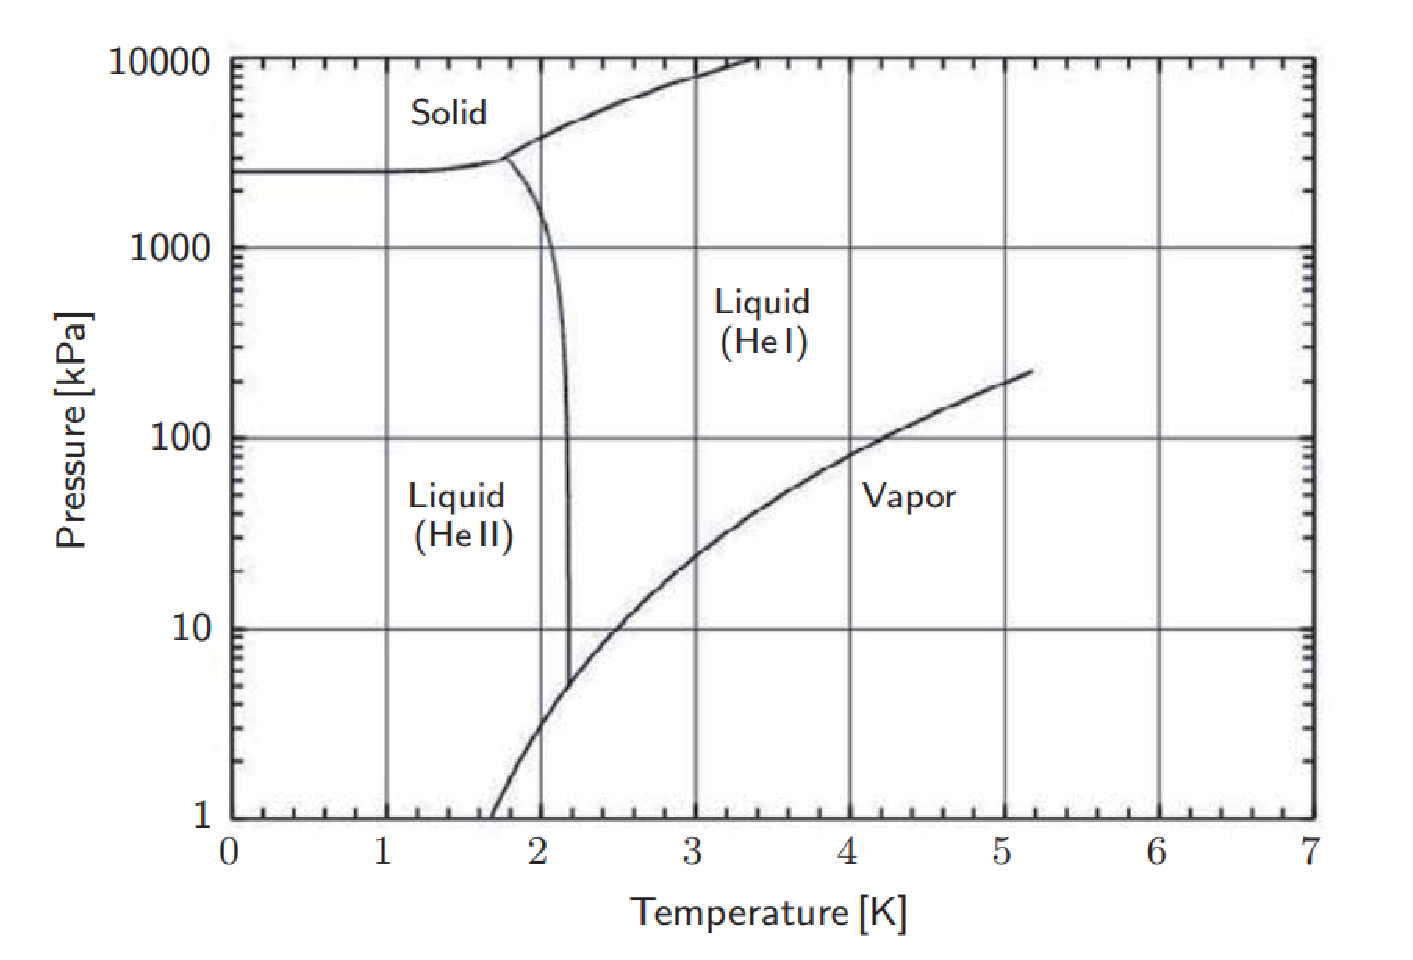
\includegraphics[scale=0.5]{chpt4/figs/fig4.8.eps}
	\caption{常规氦($He^4$)的相图。}
\end{figure}

\colorbox{red}{表4.6}

Bon Mardion、Claudet和Seyfert研究了He II通过窄通道的热流密度[4.21]。
图4.9以参数$X(T)$的形式给出了他们的结果:
\begin{equation}% 4.6a
X(T_{cl})-X(T_{wm})=q^{3.4}L
\end{equation}

式中,

\begin{equation*}% 4.6b
X(T_b)=q_{c}^{3.4}L \tag{4.6b}
\end{equation*}

\begin{figure}[htbp]
	\centering
	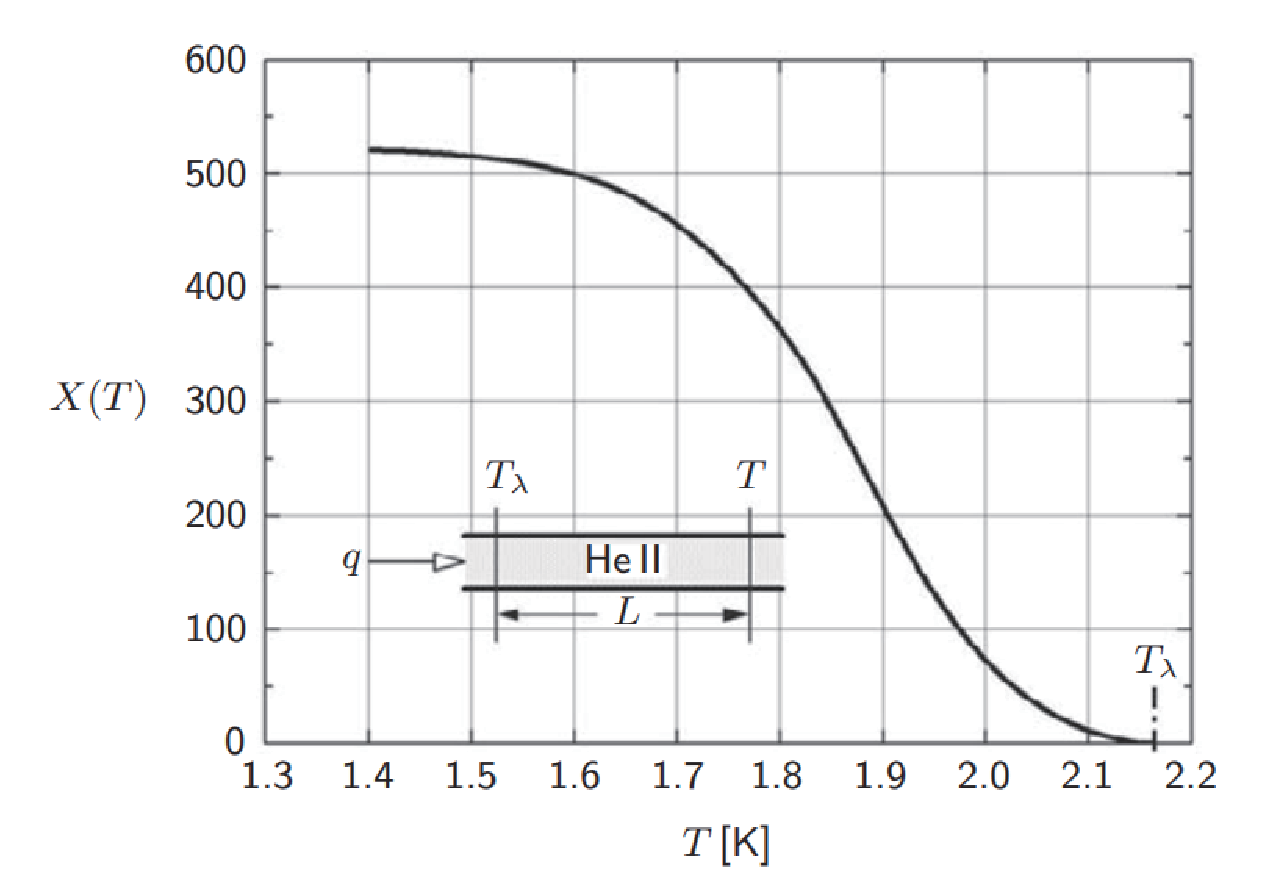
\includegraphics[scale=0.5]{chpt4/figs/fig4.9.eps}
	\caption{Bon Mardion、Claudet和Seyfert的研究结果。}
\end{figure}


\begin{equation*}% 4.6c
X(T_b)=\frac{q_{c}^{3.4}}{4.4}L \tag{4.6c}
\end{equation*}



\begin{equation}% 4.7
q_k=a_k(T_{cd}^{nk}-T_{b}^{nk})
\end{equation}

\subsection{讨论4.5:1.8 K过冷低温容器}

\begin{equation}% 4.8
Q_{out}-Q_{in}=Q_{1.8}
\end{equation}
\begin{equation}% 4.9
Q_{1.8}=\dot{m}_h(h_3-h_2)
\end{equation}

\begin{equation*}% 4.9
Q_{1.8}=\dot{m}_h(24.02J/g-5.64J/g)=20W
\end{equation*}

\begin{equation}% 4.10
P_s=Q_{1.8}=\dot{m}_h(\frac{\gamma}{\gamma-1})(P_4\nu_4)[(\frac{P_5}{P_4})^{\frac{\gamma-1}{\gamma}}-1]
\end{equation}

\begin{equation}% 4.11
T(z)=-\frac{\tilde{\rho}I_{t}^{2}}{2A^2\tilde{k}}z^2+[\frac{(T_\ell-T_0)}{\ell}+\frac{\tilde{p}I_{t}^2\ell}{2A^2\tilde{k}}]z+T_0
\end{equation}

\begin{equation}% 4.12
(\frac{I_0\ell}{A})_{dr}=\sqrt{\frac{2\tilde{k}(T_\ell-T_0)}{\dot{\rho}}}
\end{equation}

\begin{equation}% 4.13
T(\xi)=-(T_\ell-T_0)\xi^2+2(T_\ell-T_0)\xi+T_0
\end{equation}

\subsection{讨论4.6:J-T过程}

\begin{equation}% 4.14
h_g(6K,10atm)=x_\ell h_\ell(4.2K,1atm)+(1-x_\ell)h_g(4.2K,1atm)
\end{equation}

\subsection{问题4.2:基于制冷机的小型氦液化器}


\subsubsection{问题4.2之解}

\begin{equation*}% S2.1
h_{he}(7K,10atm)=x_\ell h_\ell(4.22K,1atm)+(1-x_\ell)h_v(4.22K,1atm)
\end{equation*}

\begin{equation*}% s2.2
x_\ell=\frac{h_{he}(7K,10atm)-h_v(4.22K,1atm)}{h_\ell(4.22K,1atm)-h_v(4.22K,1atm)}
=\frac{(26.00J/g-30.13J/g)}{(9.71J/g-30.13J/g)}=0.202
\end{equation*}

\begin{equation*}% S2.3
\dot{m}_{he}h_{he}(8K,10atm)=Q_2+\dot{e}_{he}h_{he}(7K,10atm)
\end{equation*}

\begin{equation*}% s2.3
Q_2=\dot{m}_{he}[h_{he}(8K,10atm)-h_{he}(7K,10atm)]
=(1g/s)(33.44J/g-26.00J/g)=7.44W
\end{equation*}

\begin{equation*}% 2.4
\dot{m}_{he}h_{he}(46K,10atm=Q_1+\dot{m}_{he}h_{he}(30K,10atm)
\end{equation*}

\begin{equation*}% S2.4
Q_1=\dot{m}[h_{he}(46K,10atm)-h_{he}(30K,10atm)]
=(1g/s)(252J/g-168J/g)\simeq84W
\end{equation*}

\begin{equation*}% S2.5
\dot{m}[h_{he}(30K,10atm)-h_{he}(8K,10atm)]
=(\dot{m}_v+\dot{m}_{\ell r})h_v(30K,1atm)-[\dot{m}_vh_v(4.22K,1atm)+\dot{m}_{\ell r}h_l(4.22K,1atm)]
\end{equation*}

\begin{equation*}% page 246
\dot{m}_{\ell r}=\frac{\{\dot{m}_{he}[h_{he}(30K,10atm)-h_{he}(8K,10atm)]-\dot{m}_v[h_v(30K,1atm)-h_{v}(4.22K,1atm)]\}}{h_v(30K,1atm)-h_{l}(4.22K,1atm)}
=\frac{(1g/s)(168.4J/g-33.44J/g)-(0.798g/s)(170.2J/g-30.13J/g)}{(170.2J/g-9.71J/g)}\simeq0.144g/s
\end{equation*}
\begin{equation*}% S2.6
\dot{m}_{\ell r}[h_{he}(295K,10atm)-h_{he}(46K,10atm)]
=(\dot{m}_v+\dot{m}_{\ell r})[h_v(295K,1atm)-h_{v}(30K,1atm)]
\end{equation*}
\begin{equation*}% S2.7a
\dot{m}_{he}[h_{he}(295K,10atm)-h_{he}(46K,10atm)]=(1g/s)(1550.0J/g-253.9J/g)
\simeq1296W
\end{equation*}
\begin{equation*}% 2.7b
(\dot{m}_v+\dot{m}_{\ell r})[h_{he}(295K,1atm)-h_{he}(30K,1atm)]
\simeq(0.798g/s+0.144g/s)(1547.0J/g-170.2J/g)
\simeq1297W/s
\end{equation*}
\begin{equation*}% s2.8
P_s=\dot{m}_h(\frac{\gamma}{\gamma-1})(P_jv_j)[(\frac{P_a}{P_j})^{\frac{\gamma-1}{\gamma}}-1]
\end{equation*}


\subsection{讨论4.7:制冷机 vs. 制冷回环器}


\subsection{讨论4.8:辐射传热}
\begin{equation}% 4.15
q_r=\epsilon_r\sigma T^4
\end{equation}
\begin{equation}% 4.16
\epsilon_r=\frac{\epsilon_{cl}\epsilon_{wm}}{\epsilon_{cl}+\epsilon_{wm}-\epsilon_{cl}\epsilon_{wm}}
\end{equation}
\begin{equation}% 4.17
q_r=\epsilon_r\sigma(T_{wm}^4-T_{cl}^4)
\end{equation}
\begin{equation}% 4.18
q_r=\frac{\epsilon_r}{N_i+1}\sigma(T_{wm}^4-T_{cl}^4)
\end{equation}



\subsection{讨论4.9:残余气体的对流传热}

\begin{equation}% 4.19
q_g=\eta_gP_g(T_{wm}-T_{cl})
\end{equation}



\subsection{讨论4.10:真空泵系统}



\subsection{讨论4.11:固态制冷工质/磁体}
\begin{equation}% 4.20
D_{th}=\frac{k}{\varrho c_p}
\end{equation}
\begin{equation}% 4.21
T_{sd}=\frac{1}{D_{th}}(\frac{\delta_{sd}}{\pi})^2
\end{equation}


\subsection{问题4.3:固态制冷剂冷却的磁体}

\begin{equation*}% page260
h(15K)-h(10K)\simeq\frac{C_p(10K)+C_p(15K)}{2}(15K-10K)
\simeq\frac{(0.175J/cm^3K+0.475J/cm^3K)}{2}(5K)
\simeq1.625J/cm^3
\end{equation*}
\begin{equation*}% page260
[\Delta(10K \rightarrow15K)]_{15liter}^{0.25W}=\frac{(15000cm^3)(1.625J/cm^3)}{(0.25W)(3600s/h)}\simeq27.1h~30h
\end{equation*}


\begin{equation*}% S3.1
\nu_{N2}=\pi D\ell\Delta r_{N2}
\Delta r_{N2}=\frac{\mu_{N2}}{\pi D\ell}=\frac{(15000cm^3)}{\pi(90cm)(30cm)}=1.8cm
\end{equation*}
\begin{equation}% 4.21
\tau_{sd}=\frac{1}{D_{th}}(\frac{\delta_{sd}}{\pi})^2
=\frac{1}{(55\times10^{-2}cm^2/s)}(\frac{1.8cm}{\pi})^2~0.6s
\end{equation}
\begin{equation*}% page260
h(15K)-h(10K)\simeq\frac{C_p(10K)+C_p(15K)}{2}(15K-10K)
\simeq\frac{(0.400J/cm^3K+0.875J/cm^3K)}{2}(5K)
\simeq3.2J/cm^3
\end{equation*}
\begin{equation*}% page261
V_{Ne}(10K \rightarrow 15K)=\frac{(27.1h)(3600s/h)(2.5W)}{(3.2J/cm^3)(1000cm^3/liter)}
\simeq7.6liter~\frac{1}{2}\times15liter
\end{equation*}
\begin{equation*}% page261
V_{Ne}(10K \rightarrow 15K)=\frac{(0.486h)}{0.89h}(15liter)\simeq8.2liter\simeq\frac{1}{2}\times(15liter)
\end{equation*}
\begin{equation*}% page261
[\Delta t(15K \rightarrow 60K)]_{15liter}^{3.3W}=(\frac{15liter}{1liter})(\frac{1W}{3.3W})[\Delta t(15K\rightarrow60K)]_{1liter}^{1W}
\simeq(15)(0.303)(17.15h)
=78h~80h
\end{equation*}
\begin{equation*}% S3.2
\int_{20K}^{T_i}[C_p(T)]_{cu}dT=5J/cm^3
\end{equation*}
\begin{equation*}% page261
h(35K)-h(30K)\simeq\frac{C_p(30K)+C_p(35K)}{2}(35K-30K)
\simeq\frac{(1.24J/cm^3K+1.55J/cm^3K)}{2}(5K)
\simeq7.0J/cm^3
\end{equation*}
\begin{equation*}% page262
[\Delta t(30K \rightarrow 35K)]_{15liter}^{10W}=\frac{(15000cm^3)(7.0J/cm^3)}{(10W)(3,600s/h)}
\simeq2.9h~3h
\end{equation*}
\begin{equation*}% page262
h(40K)-h(35K)\simeq\frac{C_p(35K)+C_p(35.61K)}{2}(35.61K-35K)
+\Delta h(35.61K)+\frac{C_p(35.61K)+C_p(40K)}{2}(40K-35.61K)
\simeq\frac{(1.60J/cm^3K+1.62J/cm^3K)}{2}(0.6K)
+8.2J/cm^3+\frac{(1.29J/cm^3K+1.33J/cm^3K)}{2}(4.39K)
\simeq0.98J/cm^3+8.2J/cm^3+5.75J/cm^3\simeq14.9J/cm^3
[\Delta t(30K \rightarrow 35K)]_{15liter}^{10W}=\frac{(15,000 cm^3)(14.9J/cm^3)}{(10W)(3,600s/h)}
\simeq6.2h~6h
\end{equation*}
\begin{equation}% 4.21
\tau_{sd}=\frac{1}{D_{th}}(\frac{\delta_{sd}}{\pi})^2
\end{equation}
\begin{equation*}% page 262
p_{sd}=[h(35K)-h(30K)]\frac{\delta_{sd}}{\tau_{sd}}
=(7.0J/cm^3)\frac{(0.04 cm)}{(0.067s)}=4.2W/cm^2
\end{equation*}



\subsection{讨论4.12:温升和场均匀性}
\begin{equation}% 4.22
\alpha(T)=\frac{1}{L_o}(\frac{\partial L}{\partial T})_P
\end{equation}
\begin{equation}% 4.23
\alpha(T)=aT+bT^3
\end{equation}
\begin{equation}% 4.24
(\frac{\Delta L}{L_o}_{cu})=\int_{10K}^{15K}(5\times10^{-9}T+3\times10^{-11}T^3)dT=0.62\times10^{-6}
\end{equation}



\subsection{讨论4.13:低温热测}




\subsection{讨论4.14:气冷铜电流引线}
\begin{equation}% 4.25
Q_{in}=[Ak(T)\frac{dT}{dz}]_{z+\Delta z}+\dot{m}_Ic_p(T)T+\frac{\rho(T)I_{o}^{2}}{A}\Delta z
\end{equation}
\begin{equation}% 4.26
Q_{out}=[Ak(T)\frac{dT}{dz}]_z+\dot{m}_Ic_p(T)(T+\Delta T)
\end{equation}
\begin{equation}% 4.27
[Ak(T)\frac{dT}{dz}]_{z+\Delta z}-[Ak(T)\frac{dT}{dz}]_z-\dot{m}_Ic_p(T)\Delta T+\frac{\rho(T)I_{o}^{2}}{A}\Delta z=0
\end{equation}
\begin{equation}% 4.28
\frac{d[Ak(T)\frac{dT}{dz}]}{dz}-\dot{m}_Ic_p(T)\frac{dT}{dz}+\frac{\rho(T)I_{o}^{2}}{A}=0
\end{equation}
\begin{equation}% 4.29a
-\dot{m}_Ic_{p0}\frac{dT}{dz}\mid_{z=0}+\frac{\rho(T)I_{o}^{2}}{A}\simeq0
\end{equation}
\begin{equation}% 4.29b
\frac{dT}{dz}\mid_{z=0}\simeq\frac{\rho_0I_{o}^{2}}{A\dot{m}_Ic_{p0}}
\end{equation}
\begin{equation}% 4.30
Q_{I_o}=Ak(T_0)\frac{dT}{dz}\mid_{z=0}=\frac{k_0\rho_0I_{0}^{2}}{\dot{m}_Ic_{p0}}
\end{equation}
\begin{equation}% 4.31a
\dot{m}_I=\frac{Q_{I_o}}{h_L}
\end{equation}
\begin{equation}% 4.31b
\dot{m}_I=I_o\sqrt{\frac{k_0\rho_0}{c_{p0}h_L}}
\end{equation}
\begin{equation}% 4.32a
\frac{Q_{I_o}}{I_o}=\sqrt{\frac{h_Lk_0\rho_0}{c_{p0}}}
\end{equation}
\begin{equation}% 4.32b
\frac{Q_{I_o}}{I_o}\simeq\sqrt{\frac{(20.7\times10^3J/kg)(600W/mK)(2.5\times10^{-10}\Omega m)}{5.26\times10^3J/kgK}}
=7.7\times10^{-4}W/A=0.77mW/A~1mW/A
\end{equation}
\begin{equation}% 4.33
\dot{m}_Ic_p(T)\frac{dT}{dz}+\frac{\rho(T)I_{o}^{2}}{A}=0
\end{equation}
\begin{equation}% 4.34a
\int_{T_o}^{T_i}\frac{dT}{\rho(T)}=\int_{0}^{\ell}\frac{I_{o}^{2}dz}{A\dot{m}_I\tilde{c}_p}=\frac{I_{o}^{2}\ell}{A\dot{m}_I\tilde{c}_p}
\end{equation}
\begin{equation}% 4.34b
\int_{T_o}^{T_i}\frac{dT}{\rho(T)}\simeq1.2\times10^{11}K\Omega m
\end{equation}
\begin{equation}% 4.34c
\int_{T_o}^{T_i}\frac{dT}{\rho(T)}\simeq(\frac{I_{o}^{2}\ell}{Ac_{p0}})\frac{1}{I_0}\sqrt{\frac{c_{p0}h_L}{k_0\rho_0}}
\end{equation}
\begin{equation}% 4.35a
(\frac{I_o\ell}{A})_{ot} \equiv \zeta_o\simeq[\int_{T_0}^{T_i}\frac{dT}{\rho_(T)}]\sqrt{\frac{c_{p0}k_0 \rho_0}{h_L}}
\end{equation}





